
%%%%%%%%%%%%%%%%%%%%%%% file typeinst.tex %%%%%%%%%%%%%%%%%%%%%%%%%
%
% This is the LaTeX source for the instructions to authors using
% the LaTeX document class 'llncs.cls' for contributions to
% the Lecture Notes in Computer Sciences series.
% http://www.springer.com/lncs       Springer Heidelberg 2006/05/04
%
% It may be used as a template for your own input - copy it
% to a new file with a new name and use it as the basis
% for your article.
%
% NB: the document class 'llncs' has its own and detailed documentation, see
% ftp://ftp.springer.de/data/pubftp/pub/tex/latex/llncs/latex2e/llncsdoc.pdf
%
%%%%%%%%%%%%%%%%%%%%%%%%%%%%%%%%%%%%%%%%%%%%%%%%%%%%%%%%%%%%%%%%%%%


\documentclass[runningheads,a4paper]{llncs}

\usepackage{xcolor} % Colors
\usepackage{pgfplots} % Bar charts
\usepackage{tikz}
\usepackage{keyval}

\usepgfplotslibrary{groupplots}

\pgfplotsset{compat=newest}
   
   
%
% Define bar chart colors
%
\definecolor{bblue}{HTML}{4F81BD}
\definecolor{rred}{HTML}{C0504D}
\definecolor{ggreen}{HTML}{9BBB59}
\definecolor{ppurple}{HTML}{9F4C7C}


\usepackage{amssymb}
\setcounter{tocdepth}{3}
\usepackage{graphicx}

\newcommand{\keywords}[1]{\par\addvspace\baselineskip
\noindent\keywordname\enspace\ignorespaces#1}

\begin{document}

\mainmatter  % start of an individual contribution

\title{A Stochastic Approach to Optimization of Deterministic Finite Automata}

% a short form should be given in case it is too long for the running head
\titlerunning{Algorithms and Computability}

\author{Jakub Ciecierski \and Bartlomiej Dybisz \\ 
\textit{Warsaw University of Technology,\\
Faculty of Mathematics and Information Science.}}
%
\authorrunning{Algorithms and Computability}

\toctitle{Algorithms and Computability}
\tocauthor{Methodology}
\maketitle

\section{Modeling}

\section{Experiments}

\subsection{Reconstruction}
\subsection{Approximation}

\section{Results}


\pgfkeys{
 /myparbox/.is family, /myparbox,
 % Here are the options that a user can pass
 default/.style = 
  {width = \textwidth, height = \baselineskip,
   position = center, inner position = center},
 width/.estore in = \myparboxWidth,
 height/.estore in = \myparboxHeight,
 position/.style = {positions/#1/.get = \myparboxPosition},
 inner position/.style = {positions/#1/.get = \myparboxInnerPos},
 % Here is the dictionary for positions.
 positions/.cd,
  top/.initial = t,
  center/.initial = c,
  bottom/.initial = b,
  stretch/.initial = s,
}

% We process the options first, then pass them to `\parbox` in the form of macros.
\newcommand\myparbox[2][]{%
 \pgfkeys{/myparbox, default, #1}%
}

 % This should print "Some text, and"
 % followed by "a box" raised about one line above the natural position
 % followed by "and more text" after a large space.
 Some text, and \myparbox[width = 50pt, height = 20pt, position = bottom, inner position = top]{a box} and more text.

 % Should look pretty much like normal text, with slight offsets down and over around the box.
 Some text, and \myparbox[width = 30pt]{a box} and more text.

 % The box should have very spread-out lines
 Some text, and
 \myparbox[width = 30pt, height = 100pt, inner position = stretch]
 {a box\par \vspace{\stretch{1}}with\par\vspace{\stretch{1}}words}
 and more text.






\newcommand{\addGroupPlot}[2]{
	\nextgroupplot[title=Class 4.1, ylabel=Accuracy]
    		% Training |w| < C    
        \addplot[style={bblue,fill=bblue,mark=none}]
            coordinates 
            {
            		(C=4, 1.0)
        			(C=5, 1.0)
       		};

    		% Training |w| > C
       	\addplot[style={rred,fill=rred,mark=none}]
            coordinates 
            {
            		(C=4, 1.0)
        			(C=5, 1.0)
       		};
       		       		
		% Training All	
        \addplot[style={ggreen,fill=ggreen,mark=none}]
            coordinates 
            {
            		(C=4, 1.0)
        			(C=5, 1.0)
       		};

		% Testing
       	\addplot[style={ppurple,fill=ppurple,mark=none}]
            coordinates 
            {
            		(C=4, 1.0)
        			(C=5, 1.0)
       		};
}









\pgfplotsset{xticklabel style={text width=2em,align=center}}

\hspace{-3.0cm}
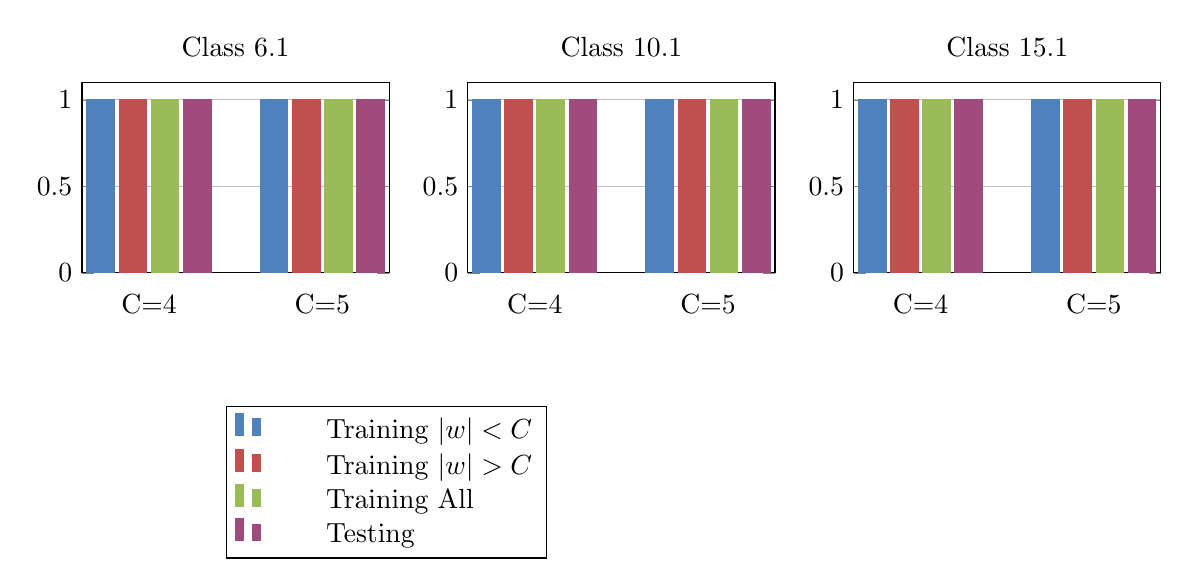
\begin{tikzpicture}


%--------------------------------------------------------------------------------------
% AXIS
%--------------------------------------------------------------------------------------

 	\begin{groupplot}[group style={group size= 4 by 3},
	    height = 4cm,
    		ybar=4*\pgflinewidth,
  		ymin=0,
    		x=2.2cm,
    		enlarge x limits={abs=0.85cm},	        
	 	major x tick style = transparent,    
       	ymajorgrids = true,
       	symbolic x coords={C=4,C=5},
        	xtick = data,
        	scaled y ticks = false,
        	legend cell align=left,
        	legend style={
                at={(-1,-1.5)},
                anchor=south east,
                column sep=5ex
        		} 	
 	]

%--------------------------------------------------------------------------------------
% CLASS 4.1
%--------------------------------------------------------------------------------------
       
\addGroupPlot{1}{2}
     	

%--------------------------------------------------------------------------------------
% CLASS 6.1
%--------------------------------------------------------------------------------------
       

     	\nextgroupplot[title=Class 6.1]
    		% Training |w| < C    
        \addplot[style={bblue,fill=bblue,mark=none}]
            coordinates 
            {
            		(C=4, 1.0)
        			(C=5, 1.0)
       		};

    		% Training |w| > C
       	\addplot[style={rred,fill=rred,mark=none}]
            coordinates 
            {
            		(C=4, 1.0)
        			(C=5, 1.0)
       		};
       		       		
		% Training All	
        \addplot[style={ggreen,fill=ggreen,mark=none}]
            coordinates 
            {
            		(C=4, 1.0)
        			(C=5, 1.0)
       		};

		% Testing
       	\addplot[style={ppurple,fill=ppurple,mark=none}]
            coordinates 
            {
            		(C=4, 1.0)
        			(C=5, 1.0)
       		};
       		
       		
       		       		%--------------------------------------------------------------------------------------
% CLASS 10.1
%--------------------------------------------------------------------------------------
       		
       		
       	\nextgroupplot[title=Class 10.1]
       	% Training |w| < C    
        \addplot[style={bblue,fill=bblue,mark=none}]
            coordinates 
            {
            		(C=4, 1.0)
        			(C=5, 1.0)
       		};

    		% Training |w| > C
       	\addplot[style={rred,fill=rred,mark=none}]
            coordinates 
            {
            		(C=4, 1.0)
        			(C=5, 1.0)
       		};
       		       		
		% Training All	
        \addplot[style={ggreen,fill=ggreen,mark=none}]
            coordinates 
            {
            		(C=4, 1.0)
        			(C=5, 1.0)
       		};

		% Testing
       	\addplot[style={ppurple,fill=ppurple,mark=none}]
            coordinates 
            {
            		(C=4, 1.0)
        			(C=5, 1.0)
       		};
       		
       		
       		
%--------------------------------------------------------------------------------------
% CLASS 15.1
%--------------------------------------------------------------------------------------
       
       
       	\nextgroupplot[title=Class 15.1]
    		% Training |w| < C    
        \addplot[style={bblue,fill=bblue,mark=none}]
            coordinates 
            {
            		(C=4, 1.0)
        			(C=5, 1.0)
       		};

    		% Training |w| > C
       	\addplot[style={rred,fill=rred,mark=none}]
            coordinates 
            {
            		(C=4, 1.0)
        			(C=5, 1.0)
       		};
       		       		
		% Training All	
        \addplot[style={ggreen,fill=ggreen,mark=none}]
            coordinates 
            {
            		(C=4, 1.0)
        			(C=5, 1.0)
       		};

		% Testing
       	\addplot[style={ppurple,fill=ppurple,mark=none}]
            coordinates 
            {
            		(C=4, 1.0)
        			(C=5, 1.0)
       		};
    
%--------------------------------------------------------------------------------------
% LEGEND
%--------------------------------------------------------------------------------------
          		
    \legend{Training $|w|<C$, Training $|w|>C$, Training All, Testing}
    \end{groupplot}

\end{tikzpicture}







\subsection{Reconstruction}
\subsection{Approximation}

\section{Appendix}

\begin{thebibliography}{4}

%\bibitem

\end{thebibliography}

\end{document}
